\documentclass[11pt, a4paper]{article}

\usepackage[utf8]{inputenc}
\usepackage{setspace}
\usepackage[margin=1in]{geometry}
\usepackage{amsmath, amssymb}
\usepackage{booktabs}
\usepackage{graphicx}
\usepackage{xcolor}
\usepackage{fancyhdr}
\usepackage{titling}
\usepackage{caption}
\usepackage[section]{placeins}
\usepackage{microtype}
\usepackage{enumitem}

\setstretch{1.15}
\emergencystretch=3em
\setlist{itemsep=1pt, topsep=3pt, leftmargin=*}
\setlist[itemize]{label=-}
\setlength{\textfloatsep}{10pt plus 2pt minus 2pt}
\renewcommand{\topfraction}{0.9}
\renewcommand{\textfraction}{0.07}
\renewcommand{\floatpagefraction}{0.8}
\graphicspath{{figs/}{eda/figs/}}
\captionsetup{font=normalsize, labelfont=bf, skip=4pt}

\usepackage{hyperref}
\hypersetup{
	colorlinks=true,
	linkcolor=black,
	urlcolor=blue,
	pdftitle={Modeling Human-Cougar Conflict and Habitat Overlap in Washington State},
	pdfpagemode=UseNone,
}

\newcommand{\subtitle}[1]{%
	\posttitle{%
		\par\end{center}
	\begin{center}\large#1\end{center}
	\vskip0.2em}%
}
\setlength{\droptitle}{-2em}
\setlength{\headheight}{14pt}

\title{\textbf{Modeling Human-Cougar Conflict and Habitat Overlap in Washington State}}
\author{Kian Giuliano\\[3pt]\href{https://github.com/kian-g/Human-Cougar-Conflict-WA-State}{https://github.com/kian-g/Human-Cougar-Conflict-WA-State}}
\date{Autumn 2026}

\pagestyle{fancy}
\fancyhf{}
\rhead{\thepage}
\lhead{Modeling Human-Cougar Conflict}
\renewcommand{\headrulewidth}{0.4pt}

\fancypagestyle{plain}{%
	\fancyhf{}%
	\cfoot{\thepage}%
	\renewcommand{\headrulewidth}{0pt}%
}

\begin{document}
\maketitle
\thispagestyle{plain}

\section{Research Questions}
\begin{description}[leftmargin=2em, labelwidth=1.5em, itemsep=1em, parsep=0pt]
  \item[\textbf{RQ1:}] How does the frequency of Global Biodiversity Information Facility (GBIF) cougar occurrences and Washington Department of Fish and Wildlife (WDFW) dangerous-incident reports vary with distance to the nearest Wildland-Urban Interface (WUI) area and the nearest county road, and do records inside WUI zones lie significantly closer to roads than records in wildland areas?

  \item[\textbf{RQ2:}] Across a $5\text{ km} \times 5\text{ km}$ grid of Washington State, is there an inverse relationship or threshold between county road density and cougar occurrences per cell, suggesting that dense road networks act as barriers?

  \item[\textbf{RQ3:}] Can a machine learning classifier predict whether a grid cell contains a cougar occurrence from its road density, WUI classification, and structure density?
\end{description}

\section{Motivation}
Suburban growth in Washington State is expanding the Wildland-Urban Interface (WUI), where development meets undeveloped vegetation, and bringing cougars (\textit{Puma concolor}) into closer contact with people, pets, and livestock.\footnote{\href{https://doi.org/10.1073/pnas.1718850115}{Radeloff et al., \textit{PNAS}, 2018}; \href{https://doi.org/10.1890/11-0947.1}{Kertson et al., \textit{Ecol.\ Appl.}, 2011}.} Wildlife managers mostly respond after a conflict has already happened.\footnote{\href{https://doi.org/10.1371/journal.pone.0079713}{Peebles et al., \textit{PLoS ONE}, 2013}; \href{https://doi.org/10.1644/12-MAMM-A-051.1}{Kertson et al., \textit{J.\ Mammal.}, 2013}.} If roads, housing density, and habitat edges predict where cougars are seen and where conflicts occur, managers could act earlier. RQ1 asks whether conflict concentrates where roads give people access to habitat edges. RQ2 asks whether road networks break up cougar habitat, which would affect where corridors and crossings are built. RQ3 asks whether these features can flag high-risk areas in advance, so that outreach such as livestock fencing and pet guidance goes where it is most needed.

\section{Dataset}
All four datasets are public, and none need an account. (The code also downloads the Census 1:20M state outline automatically the first time it runs). To reproduce the analysis, clone the repository and follow the steps below. \texttt{run\_eda.py} does all cleaning in code.
\begin{enumerate}
  \item \textbf{\href{https://www.gbif.org/occurrence/search?taxonKey=4QHKG&taxonKey=5KSLV&taxonKey=5KSLR&hasCoordinate=true&hasGeospatialIssue=false&country=US}{GBIF occurrences}}: museum, research, and iNaturalist records of \textit{Puma concolor}. No manual download is needed: the code queries the \href{https://api.gbif.org/v1/occurrence/search}{GBIF API} for Washington's bounding box (the linked search page shows the whole US) in pages of 300 records and caches the result to \texttt{data/gbif\_cougar\_wa.csv}.
  \item \textbf{\href{https://wdfw.maps.arcgis.com/apps/webappviewer/index.html?id=35dae8aafe84486d8aaef1a4b74a87e1}{WDFW Dangerous Incident Reports}}: incidents before August 1, 2022, filtered to cougars and exported as \texttt{Dangerous Incidents - Cougar.csv}. The web map has no direct download, so the exported CSV is included in the repository's \texttt{data/} folder.
  \item \textbf{\href{https://data-wadnr.opendata.arcgis.com/maps/581ce1cdcf0c46f0b39dc3264ec05d96/about}{Washington Department of Natural Resources (WADNR) Wildland-Urban Interface (2019)}}: a 30 m GeoTIFF raster with 16 classes. Download the zipped raster from the linked page and unzip it to \texttt{data/wui\_wa\_tif/} (so the raster is \texttt{data/wui\_wa\_tif/wui.tif}).
  \item \textbf{\href{https://geo.wa.gov/datasets/93b79a6fa8554e19b462a2905cbcc314_0/}{Washington State Department of Transportation (WSDOT) County Roads (2024)}}: every public county road, as reported to the County Road Administration Board (CRAB). Choose \emph{Download} $\rightarrow$ \emph{GeoJSON} on the linked page and save it as \texttt{data/WSDOT\_-\_County\_Road\_(CRAB).geojson}.
\end{enumerate}

\section{Method}
\label{sec:method}
\textbf{EDA steps.} I projected each layer to WA State Plane South (EPSG:2927), the raster's native coordinate reference system (CRS), and report distances in meters. For each dataset I computed its size, missing values (\texttt{isna().sum()}), and summaries (\texttt{describe()}, \texttt{value\_counts()}), and made at least two plots. I then joined the layers. Each point gets the WUI class of its 30 m cell (\texttt{rasterio}), grouped as \emph{WUI} (classes 7--14), \emph{Wildland} (1, 99), or \emph{Other}. It also gets its distance to WUI (a \texttt{scipy.ndimage} distance transform on a 120 m copy of the raster) and to the nearest road (\texttt{sjoin\_nearest}). Finally, a 5 km grid (7,254 cells with at least 25\% land) gets road density (\texttt{overlay}) and point counts (\texttt{sjoin}).

\medskip
\noindent\textbf{RQ1 (planned).} Count GBIF and WDFW records per band of \texttt{dist\_to\_wui\_m} and \texttt{dist\_to\_road\_m} (0, 0--250 m, 250 m--1 km, 1--5 km, $>$5 km), with WDFW split into sightings and conflicts. Compare \texttt{dist\_to\_road\_m} for WUI and Wildland records with the tests in Section~\ref{sec:joined}, then repeat on three subsets: GBIF records located to within 1 km, one record per 5 km cell, and confirmed WDFW reports. The effect size is the median difference and the rank-biserial correlation.

\medskip
\noindent\textbf{RQ2 (planned).} Spearman's $\rho$ between \texttt{road\_density\_km2} and \texttt{cougar\_count}, and with \texttt{incident\_count} for comparison (leaving out the four counties WDFW does not cover), with a permutation $p$-value. Shares of occupied cells per density bin will show any threshold, and a Plotly map will show the grid. A negative $\rho$ or a drop in occupancy at high density supports the barrier hypothesis. A positive $\rho$ more likely reflects reporting effort.

\medskip
\noindent\textbf{RQ3 (planned).} A cell is positive if \texttt{cougar\_count} $\ge 1$ (259 cells, 3.6\%). The features are \texttt{road\_density\_km2}, the cell's WUI share, and its structure-density level from \texttt{WUI\_DESC\_N}. On a stratified 80/20 split, \texttt{GridSearchCV} (5-fold, balanced class weights, \texttt{average\_precision}) tunes a Random Forest and a support vector machine (SVM) with a radial basis function (RBF) kernel, and the best model is compared with a \texttt{DummyClassifier} by the area under the ROC curve (ROC-AUC) and under the precision-recall curve (PR-AUC). The two WUI features are correlated, so permutation importance shuffles them as one group. A high PR-AUC would show where cougars are \emph{recorded}, which is biased toward where people are.

\section{EDA Results}
Each section below is produced by \texttt{run\_eda.py}, which uses four analysis modules: \texttt{cougar\_data} (loading, cleaning, and summaries), \texttt{spatial} (joins and the grid), \texttt{validity} (assumption checks), and \texttt{figures} (one function per figure), plus \texttt{plot\_style} for shared figure styling. The figures are drawn with \texttt{matplotlib}, \texttt{seaborn}, and \texttt{geopandas}. Table~\ref{tab:seven} gives seven-number summaries of each quantitative variable of interest.

\begin{table}[!htb]
  \centering
  \caption{Seven-number summaries of quantitative variables of interest (distances in meters; SD is the standard deviation, Q1 and Q3 the first and third quartiles).}
  \label{tab:seven}
  \setlength{\tabcolsep}{4pt}
  \begin{tabular}{lrrrrrrrr}
    \toprule
    Variable                         & $n$    & Mean   & SD     & Min    & Q1     & Median & Q3     & Max     \\
    \midrule
    GBIF \texttt{year}               & 389    & 2012.8 & 24.8   & 1901   & 2018   & 2023   & 2025   & 2026    \\
    GBIF uncertainty (m)             & 352    & 11,087 & 24,833 & 0.7    & 31     & 754    & 26,679 & 345,706 \\
    GBIF latitude ($^\circ$N)        & 396    & 47.83  & 0.77   & 45.60  & 47.29  & 48.01  & 48.43  & 48.98   \\
    GBIF longitude ($^\circ$W)       & 396    & 121.02 & 2.24   & 117.10 & 119.06 & 121.91 & 122.74 & 124.64  \\
    WDFW incident year               & 4,954  & 2019.5 & 1.6    & 2016   & 2018   & 2020   & 2021   & 2022    \\
    WDFW latitude ($^\circ$N)        & 4,954  & 47.61  & 0.72   & 46.08  & 47.06  & 47.66  & 48.11  & 49.00   \\
    WDFW longitude ($^\circ$W)       & 4,954  & 120.50 & 2.27   & 117.03 & 117.94 & 120.61 & 122.59 & 124.53  \\
    Road segment \texttt{length\_m}  & 58,243 & 1,236  & 3,083  & 11.7   & 139    & 331    & 870    & 86,202  \\
    Cell \texttt{road\_density\_km2} & 7,254  & 0.40   & 0.63   & 0      & 0      & 0.22   & 0.59   & 8.90    \\
    Cell \texttt{cougar\_count}      & 7,254  & 0.055  & 0.44   & 0      & 0      & 0      & 0      & 24      \\
    Cell \texttt{incident\_count}    & 7,254  & 0.68   & 2.20   & 0      & 0      & 0      & 0      & 59      \\
    GBIF \texttt{dist\_to\_road\_m}  & 396    & 2,307  & 3,911  & 0.8    & 249    & 695    & 2,563  & 35,380  \\
    GBIF \texttt{dist\_to\_wui\_m}   & 396    & 1,856  & 3,498  & 0      & 0      & 433    & 2,340  & 35,167  \\
    WDFW \texttt{dist\_to\_road\_m}  & 4,954  & 333    & 991    & 0      & 3.4    & 41     & 311    & 25,389  \\
    WDFW \texttt{dist\_to\_wui\_m}   & 4,954  & 96     & 727    & 0      & 0      & 0      & 0      & 25,743  \\
    \bottomrule
  \end{tabular}
\end{table}

\subsection{WDFW dangerous incidents}

\begin{description}[leftmargin=0pt, itemsep=4pt]

  \item[Size:] 4,954 rows (one per reported incident, Oct.\ 2016--Jul.\ 2022)
    $\times$ 11 columns: \texttt{Incident Date}, \texttt{Species Name},
    \texttt{County}, \texttt{WDFW Region} (the agency's administrative region, 1--6), \texttt{Incident Type},
    \texttt{Confirmation Code} (WDFW's verification status), \texttt{Incident ID}, \texttt{Incident Notes},
    \texttt{Report Date}, and \texttt{x}/\texttt{y} (Web Mercator coordinates, which I convert to
    latitude/longitude).

  \item[Missing:] \texttt{Incident ID} 28 (0.57\%), \texttt{Incident Type} 25
    (0.50\%), \texttt{Incident Notes} 20 (0.40\%), \texttt{Confirmation Code} 14
    (0.28\%), \texttt{Report Date} 11 (0.22\%). No coordinates are missing.
    Rows without a type are left out of type-specific analyses only. Six rows (0.1\%) are exact duplicates, which I keep for now.
    Coverage is incomplete in the south: no incident lies south of 46.08$^\circ$N, and Clark, Skamania, Klickitat, and San Juan counties have no reports, so zero counts there mean ``unknown'' rather than ``none''.

  \item[Variables of interest:]
    \texttt{x}/\texttt{y} locate each incident for the distance joins in RQ1 and the grid counts in RQ2.
    \texttt{Incident Type} splits RQ1 into sightings and conflicts, since conflicts are what managers act on.
    \texttt{Confirmation Code} measures reliability; RQ1 is rerun on confirmed reports only.

  \item[Summaries:] Counts for the two categorical variables of interest are
    in Table~\ref{tab:wdfw-summary}. \texttt{County} takes 35 values, led by
    Spokane (571), Stevens (439), and Chelan (383). Stevens also has the most
    livestock/pet losses (144) and human-safety confrontations (33). The full
    list and a county-by-type heatmap are in Appendix~\ref{app:counties}.

\end{description}

\begin{table}[!htb]
  \centering
  \caption{Category counts in the WDFW dangerous-incidents data (code prefixes such as \texttt{SIGHT2:} omitted; 25 missing types and 14 missing codes not shown).}
  \label{tab:wdfw-summary}
  \begin{tabular}{@{}llr@{}}
    \toprule
    Variable & Value                                   & Count \\
    \midrule
    \texttt{Incident Type}
             & Sighting                                & 3,650 \\
             & Livestock or Pet Injury/Loss            & 1,121 \\
             & Human Safety Confrontation              & 158   \\
    \midrule
    \texttt{Confirmation Code}
             & Unconfirmed Sighting                    & 2,663 \\
             & Confirmed Sighting                      & 987   \\
             & Confirmed Depredation                   & 673   \\
             & Conf.\ Depredation with Removal         & 171   \\
             & Conf.\ Depredation, Other Cause/Species & 164   \\
             & Human Safety Confrontation              & 145   \\
             & Unconfirmed                             & 137   \\
    \bottomrule
  \end{tabular}
\end{table}

\begin{figure}[!htb]
  \centering
  \begin{minipage}[t]{0.42\textwidth}\vspace{0pt}
    \centering
    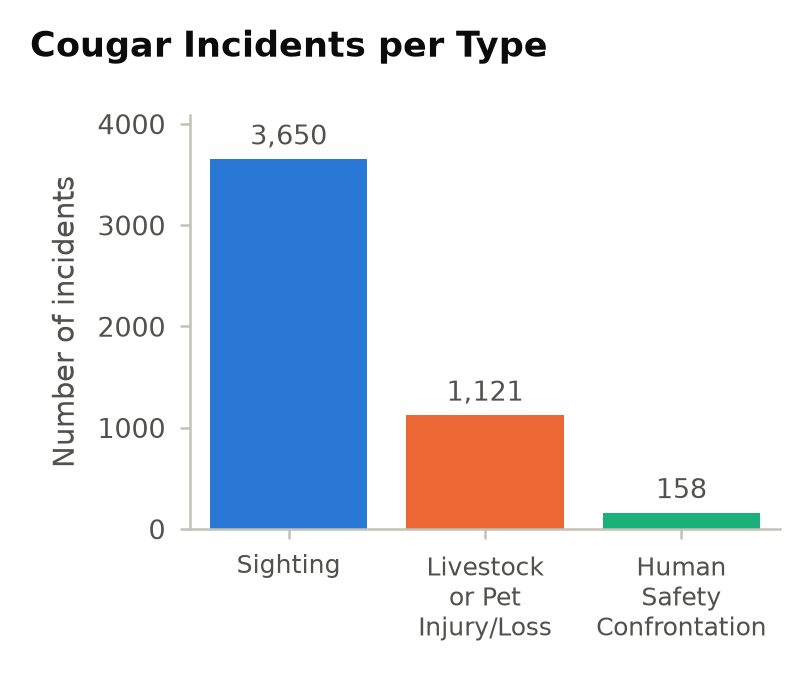
\includegraphics[width=\linewidth]{cougar_incidents_per_type.png}
  \end{minipage}\hfill
  \begin{minipage}[t]{0.56\textwidth}\vspace{0pt}
    \centering
    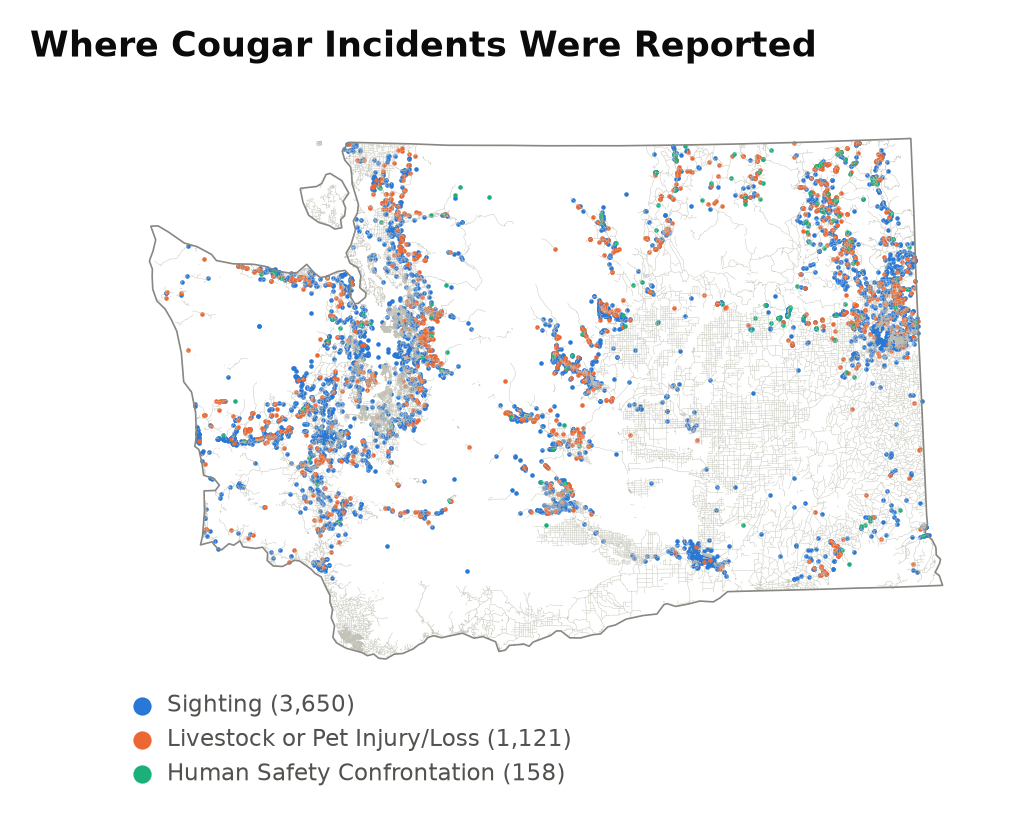
\includegraphics[width=\linewidth]{incidents_map_by_type.png}
  \end{minipage}
  \par
  \begin{minipage}[t]{0.42\textwidth}
    \caption{Sightings dominate WDFW reports; only 1,279 involve livestock, pets, or people.}
    \label{fig:types}
  \end{minipage}\hfill
  \begin{minipage}[t]{0.56\textwidth}
    \caption{Incidents cluster in foothills and valleys near development.}
    \label{fig:incmap}
  \end{minipage}
\end{figure}
Figure~\ref{fig:types} is a bar chart because that compares the sizes of a few categories most directly. Conflict records are a minority, and 2,663 of the sightings are unconfirmed. Figure~\ref{fig:incmap} maps every incident in the same type colors over the county roads, since each RQ depends on location. Cougar reports follow settled valleys and foothills (northeast Washington, the Cascade foothills, the Olympic Peninsula edge) rather than spreading across the state. The empty southern strip, including the dense road network around Vancouver, reflects the coverage gap noted above rather than an absence of cougars.

\subsection{GBIF cougar occurrences}
\begin{sloppypar}
  \begin{description}[leftmargin=0pt, itemsep=4pt]

    \item[Size:] 481 records in the bounding box, of which 396 are inside
      Washington (the other 85 are in Oregon, Idaho, or British Columbia; the
      fossil filter removed none). The data has 396 rows (one per occurrence)
      $\times$ 9 columns: \texttt{gbifID}, \texttt{decimalLongitude},
      \texttt{decimalLatitude}, \texttt{year}, \texttt{month},
      \texttt{basisOfRecord}, \texttt{datasetName}, \texttt{institutionCode},
      \texttt{coordinateUncertaintyInMeters} (the location uncertainty of each record).

    \item[Missing:] \texttt{year} 7 (1.8\%), \texttt{month} 13 (3.3\%),
      \texttt{coordinateUncertaintyInMeters} 44 (11.1\%), \texttt{datasetName}
      86 (21.7\%), \texttt{institutionCode} 3 (0.76\%). No coordinates are missing. Records without a year stay in spatial work, and records without
      an uncertainty value are left out of the precise-location check.

    \item[Variables of interest:]
      The coordinates locate each record for every join (RQ1--RQ3).
      \texttt{coordinateUncertaintyInMeters} selects the precisely located records for the RQ1 check.
      \texttt{basisOfRecord} removes fossils and shows how much of the data is opportunistic observation.
      \texttt{year} shows whether records come from roughly the same period as the 2019 WUI and 2024 road layers.

    \item[Summaries:] Quantitative variables are in Table~\ref{tab:seven}.
      \texttt{basisOfRecord}: Human Observation 308 (all iNaturalist),
      Preserved Specimen 87, Material Citation 1. Location precision is poor: 41\% of all records (46\% of the 352 with a
      recorded uncertainty) are uncertain by more than 1 km, and 30\% (34\%) by
      more than 5 km.

  \end{description}
\end{sloppypar}

\begin{figure}[!htb]
  \centering
  \begin{minipage}[t]{0.49\textwidth}\vspace{0pt}
    \centering
    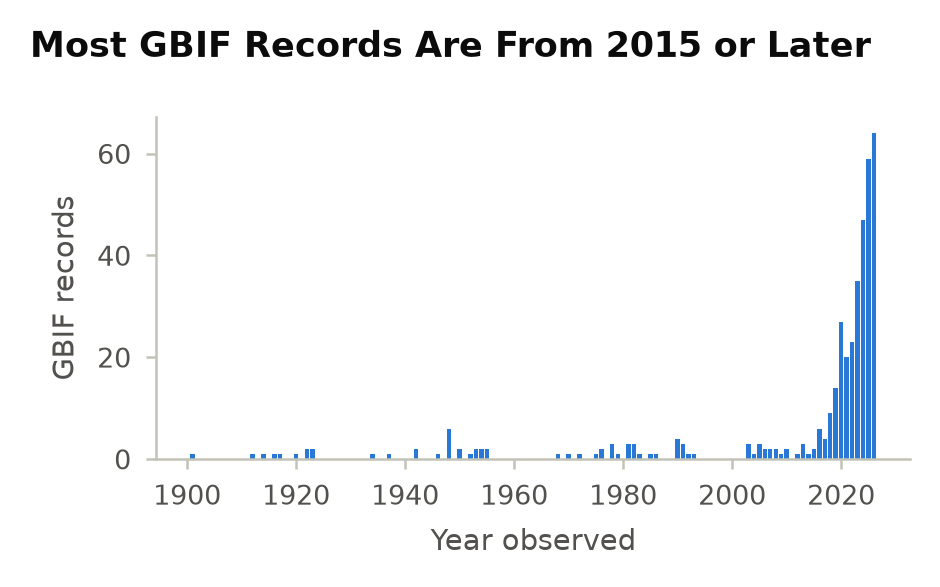
\includegraphics[width=\linewidth]{gbif_records_by_year.png}
  \end{minipage}\hfill
  \begin{minipage}[t]{0.49\textwidth}\vspace{0pt}
    \centering
    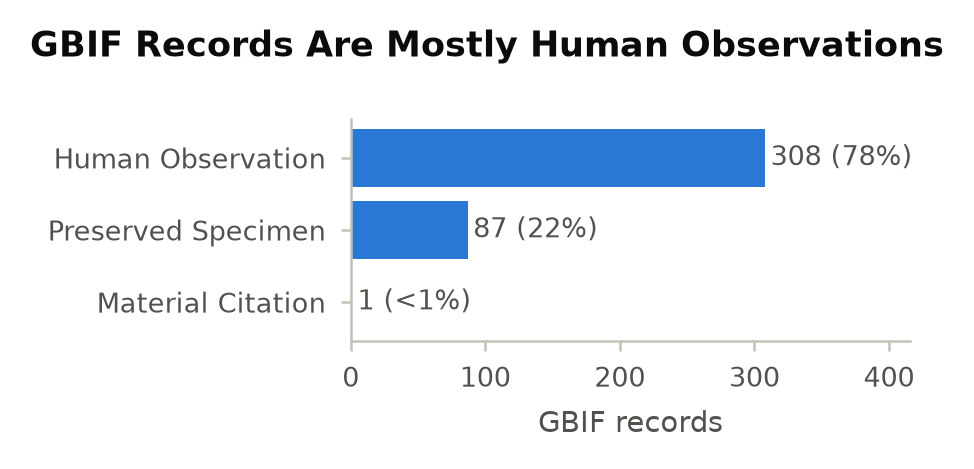
\includegraphics[width=\linewidth]{gbif_basis_of_record.png}
  \end{minipage}
  \par
  \begin{minipage}[t]{0.49\textwidth}
    \caption{78\% of GBIF records date from 2015 or later.}
    \label{fig:gbifyear}
  \end{minipage}\hfill
  \begin{minipage}[t]{0.49\textwidth}
    \caption{Most records are opportunistic human observations.}
    \label{fig:gbifbasis}
  \end{minipage}
\end{figure}

Figure~\ref{fig:gbifyear} uses one bar per year so that both the long, sparse history and the recent surge are visible on a single axis. The old records are scattered museum specimens, and the steep rise after 2015 follows iNaturalist's growth, which overlaps the WDFW period and the WUI and road layers. Figure~\ref{fig:gbifbasis} is a horizontal bar chart so the category names fit, and it shows that 308 of the 396 records are human observations. So GBIF shows where people \emph{see} cougars, and I will interpret RQ1--RQ3 with that in mind.

\subsection{WADNR Wildland-Urban Interface raster}
\begin{description}[leftmargin=0pt, itemsep=4pt]

  \item[Size:] 12,943 $\times$ 20,061 cells of 30 m. The attribute table has
    16 rows (one per class) $\times$ 3 columns: \texttt{VALUE},
    \texttt{WUI\_DESC\_N}, \texttt{COUNT}.

  \item[Missing:] The 21\% of cells outside the state border are NoData (255),
    which is expected for a rectangular raster. Inside the state there are no
    gaps. Asserts in \texttt{cougar\_data.check\_wui\_complete} (using
    \texttt{np.bincount} over all 259.6 million cells, run by both
    \texttt{run\_eda.py} and \texttt{test\_eda.py}) confirm that every cell is
    either one of the 16 classes or NoData, and the class counts sum to
    184,633 km$^2$, about 0.1\% below Washington's area.

  \item[Variable of interest:] \texttt{WUI\_DESC\_N}, the WUI classification. It gives each record's WUI group in RQ1 and the WUI share and structure-density features in RQ3.

  \item[Summary:] Figure~\ref{fig:wuibar} lists all 16 classes with their
    cell counts and shares. Vegetated Uninhabited covers 59.4\% of the state, Intermix 10.2\%,
    and Interface 2.0\%.

\end{description}

\begin{figure}[!htb]
  \centering
  \begin{minipage}[t]{0.46\textwidth}\vspace{0pt}
    \centering
    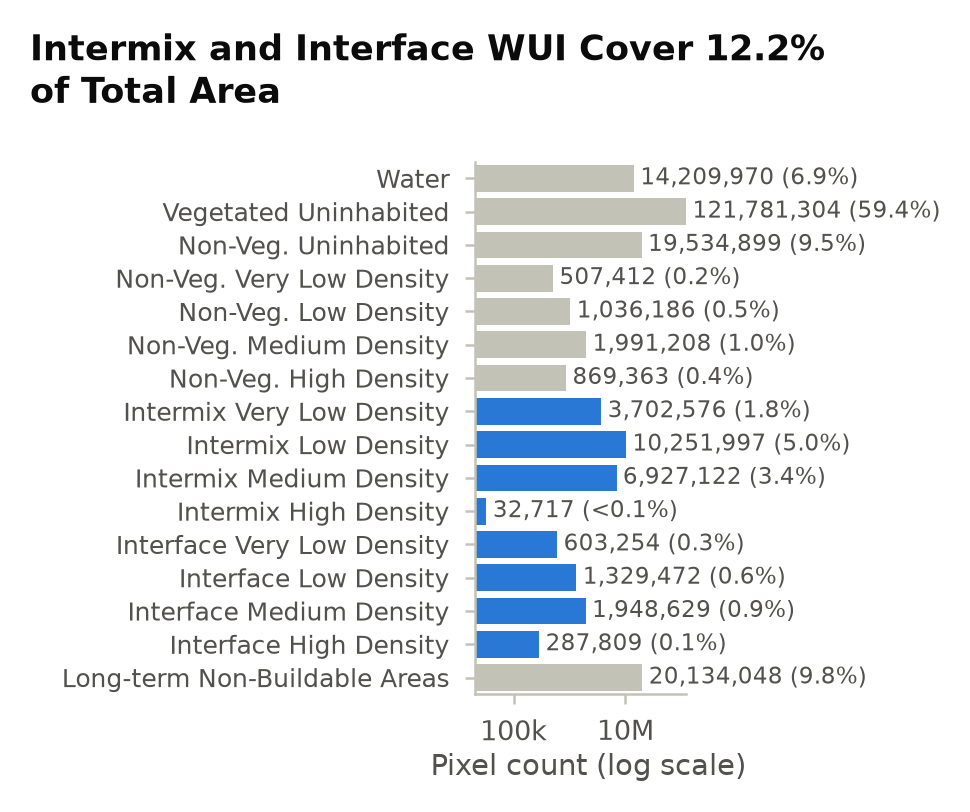
\includegraphics[width=\linewidth]{px_count_wui.png}
  \end{minipage}\hfill
  \begin{minipage}[t]{0.52\textwidth}\vspace{0pt}
    \centering
    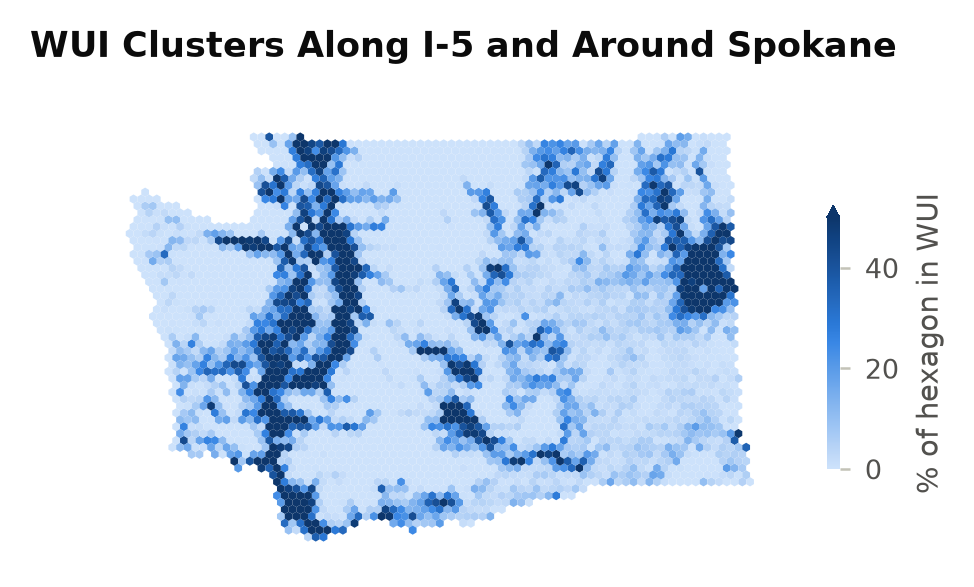
\includegraphics[width=\linewidth]{wui_hexbin.png}
  \end{minipage}
  \par
  \begin{minipage}[t]{0.46\textwidth}
    \caption{Intermix and Interface WUI cover only 12.2\% of Washington.}
    \label{fig:wuibar}
  \end{minipage}\hfill
  \begin{minipage}[t]{0.52\textwidth}
    \caption{WUI forms corridors along Interstate 5 (I-5) and eastern river valleys, and a cluster around Spokane.}
    \label{fig:wuihex}
  \end{minipage}
\end{figure}

Figure~\ref{fig:wuibar} is a bar chart on a log scale, because class sizes range from 32,717 to 122 million cells and a linear axis would hide the small WUI classes. WUI classes are blue and the rest grey, and each bar is labeled with its exact count and share. Excluding water (6.9\% of cells), where no record can fall, WUI covers 13.1\% of the state. This is the baseline for RQ1: an even spread of records would put about 13\% in the WUI. Figure~\ref{fig:wuihex} is a hexbin map of a 300 m downsampled copy of the raster (about 2 million cells, too many to draw one by one), colored by the percentage of WUI per hexagon, which shows where WUI is concentrated. Several of those areas, including Spokane and King counties, also have many incident reports (Table~\ref{tab:counties}).

\subsection{WSDOT county road network}
\begin{sloppypar}
  \begin{description}[leftmargin=0pt, itemsep=4pt]

    \item[Size:] 58,243 rows (one per road segment) $\times$ 7 columns:
      \texttt{OBJECTID}, \texttt{RouteIdentifier} and \texttt{RoadNumber} (identify each road),
      \texttt{LRSDate} (the date the road log is valid, 2024-12-31 for every row), \texttt{CountyFIPSLongPlaceCode} (the county), \texttt{GlobalID},
      \texttt{SHAPE\_Length}.

    \item[Missing:] Only \texttt{RoadNumber} (19 rows, 0.03\%, not used). A check on
      \texttt{geometry.isna()} and \texttt{is\_empty} finds no missing or empty geometries, and \texttt{length\_m} is non-null and positive for all
      58,243 rows.

    \item[Variables of interest:] The geometry, from which I derive
      \texttt{length\_m} (\texttt{SHAPE\_Length} is in degrees), \texttt{dist\_to\_road\_m} for RQ1, and per-cell \texttt{road\_density\_km2} for RQ2 and RQ3.

    \item[Summaries:] Quantitative variables are in Table~\ref{tab:seven}. The
      network totals 71,963 km, and 35\% of grid cells have no county road.

  \end{description}
\end{sloppypar}

\begin{figure}[!htb]
  \centering
  \begin{minipage}[t]{0.5\textwidth}\vspace{0pt}
    \centering
    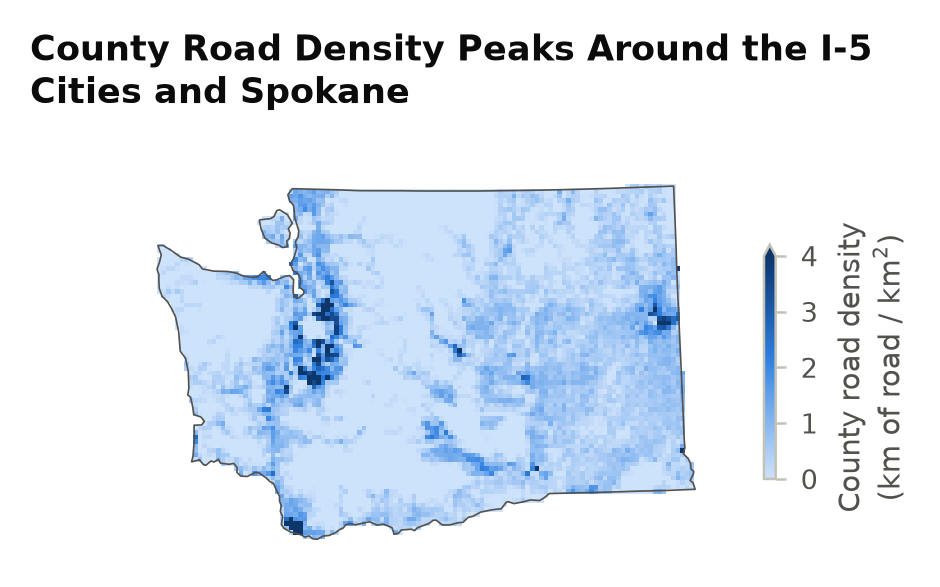
\includegraphics[width=\linewidth]{road_density_grid.png}
  \end{minipage}\hfill
  \begin{minipage}[t]{0.48\textwidth}\vspace{0pt}
    \centering
    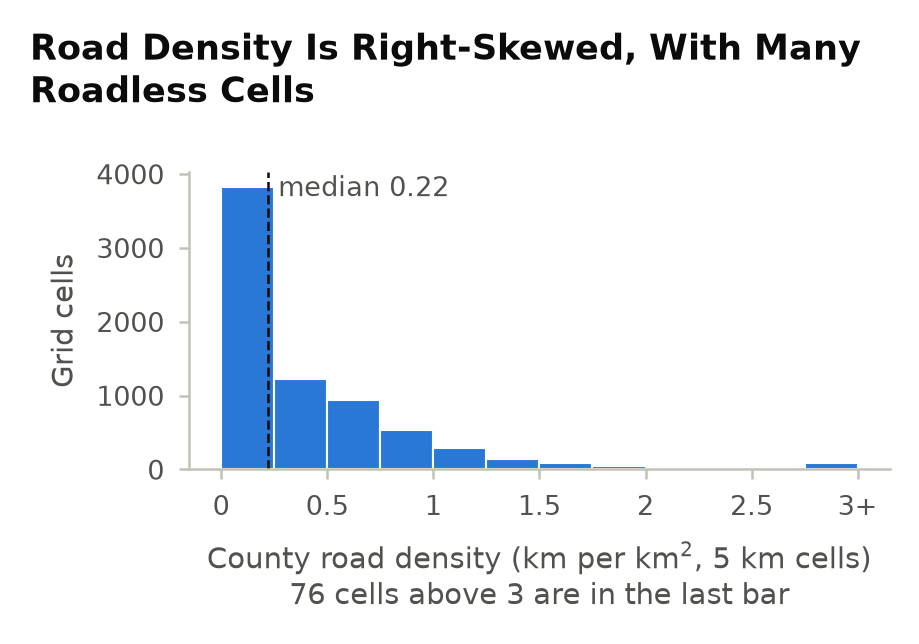
\includegraphics[width=\linewidth]{road_density_hist.png}
  \end{minipage}
  \par
  \begin{minipage}[t]{0.5\textwidth}
    \caption{County roads ring the I-5 cities (Puget Sound and Vancouver) and Spokane; city cores are gaps because city streets are excluded.}
    \label{fig:roadmap}
  \end{minipage}\hfill
  \begin{minipage}[t]{0.48\textwidth}
    \caption{Road density per cell is strongly right-skewed (median 0.22 km/km$^2$).}
    \label{fig:roadhist}
  \end{minipage}
\end{figure}

Figure~\ref{fig:roadmap} maps \texttt{road\_density\_km2} on the 5 km grid used by RQ2 and RQ3, which checks that the clipping looks right. The densest cells form rings around cities, and the eastern farm grid has moderate, even density. Figure~\ref{fig:roadhist} is a histogram, which shows the shape of a single quantitative variable best. Most cells are near zero, with a long right tail. Because of this skew, RQ2 uses Spearman's rank correlation rather than Pearson's.

\subsection{Joined data and Result Validity checks}
\label{sec:joined}
\textbf{WUI group of each record.} GBIF: Wildland 247, WUI 116, Other 33. WDFW: WUI 4,240 (85.6\%), Other 459, Wildland 253, no data 2.
Since WUI is only 13.1\% of the non-water area, WDFW incidents are about 6.5 times more concentrated in the WUI than an even spread would give (GBIF: 29\%, about 2.2 times). On the grid, only 259 of 7,254 cells (3.6\%) contain a GBIF record, so RQ3 has a strong class imbalance.

\begin{figure}[!htb]
  \centering
  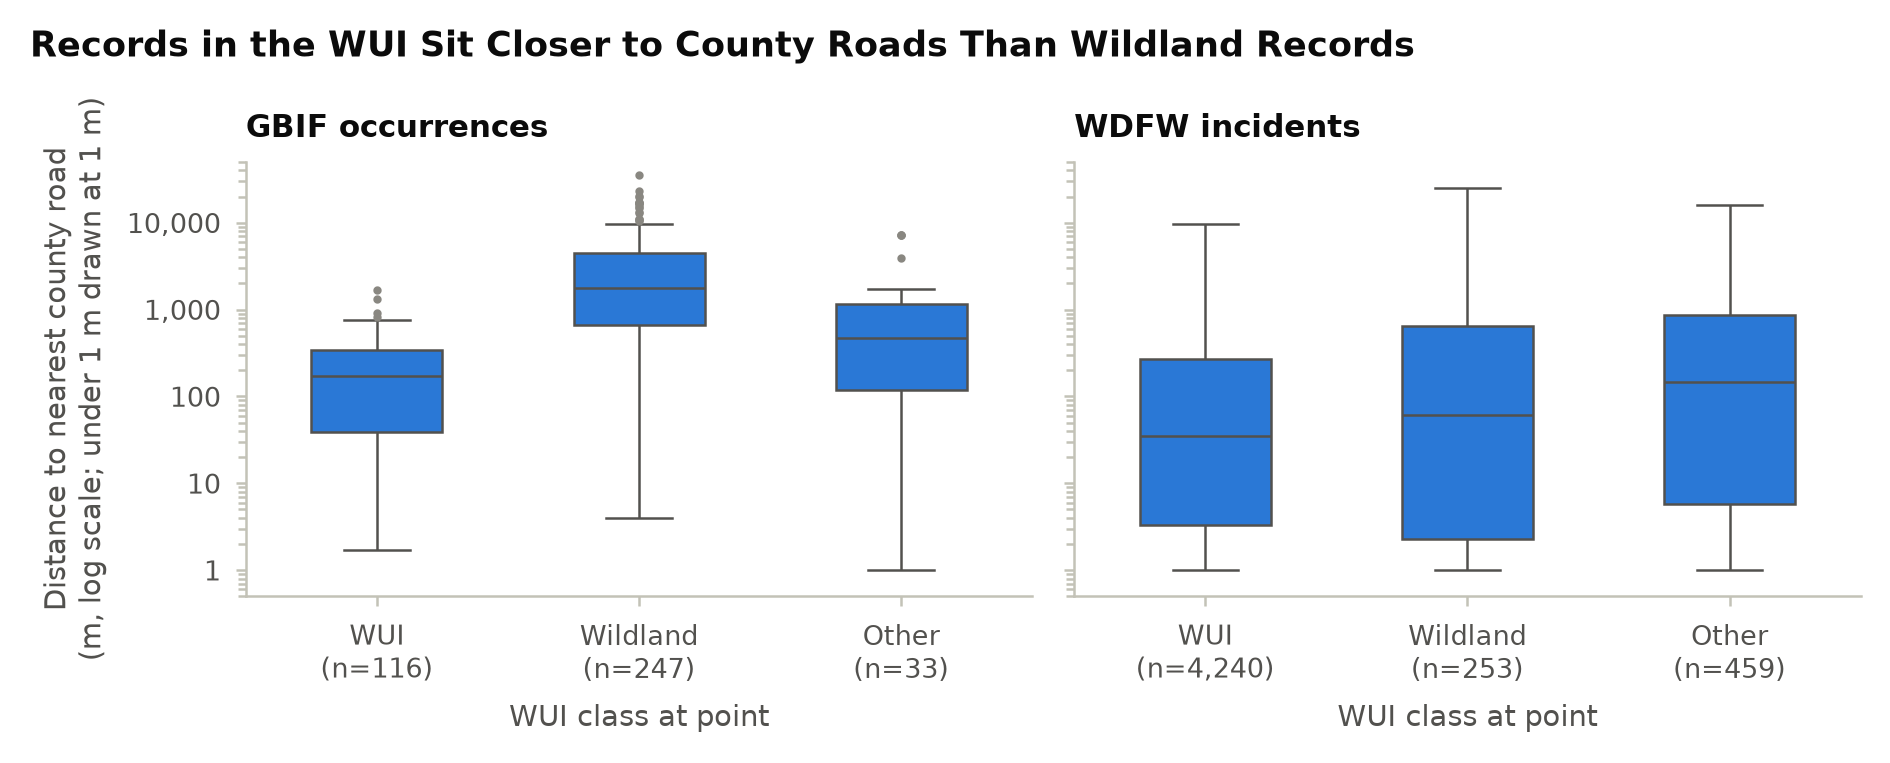
\includegraphics[width=\textwidth]{dist_to_road_by_wui.png}
  \caption{GBIF records in the WUI sit a median 171 m from a county road versus 1,780 m for wildland records; WDFW incidents are close to roads in every class.}
  \label{fig:box}
\end{figure}

Figure~\ref{fig:box} previews RQ1 with log-scale box plots, which show the medians, spreads, and outliers side by side. The GBIF gap holds for records located to within 1 km (234 m vs.\ 1,113 m, $n$=55 and 115). For WDFW, every group is close to roads (medians 35--145 m), as expected, since people report incidents where they are.

\begin{figure}[!htb]
  \centering
  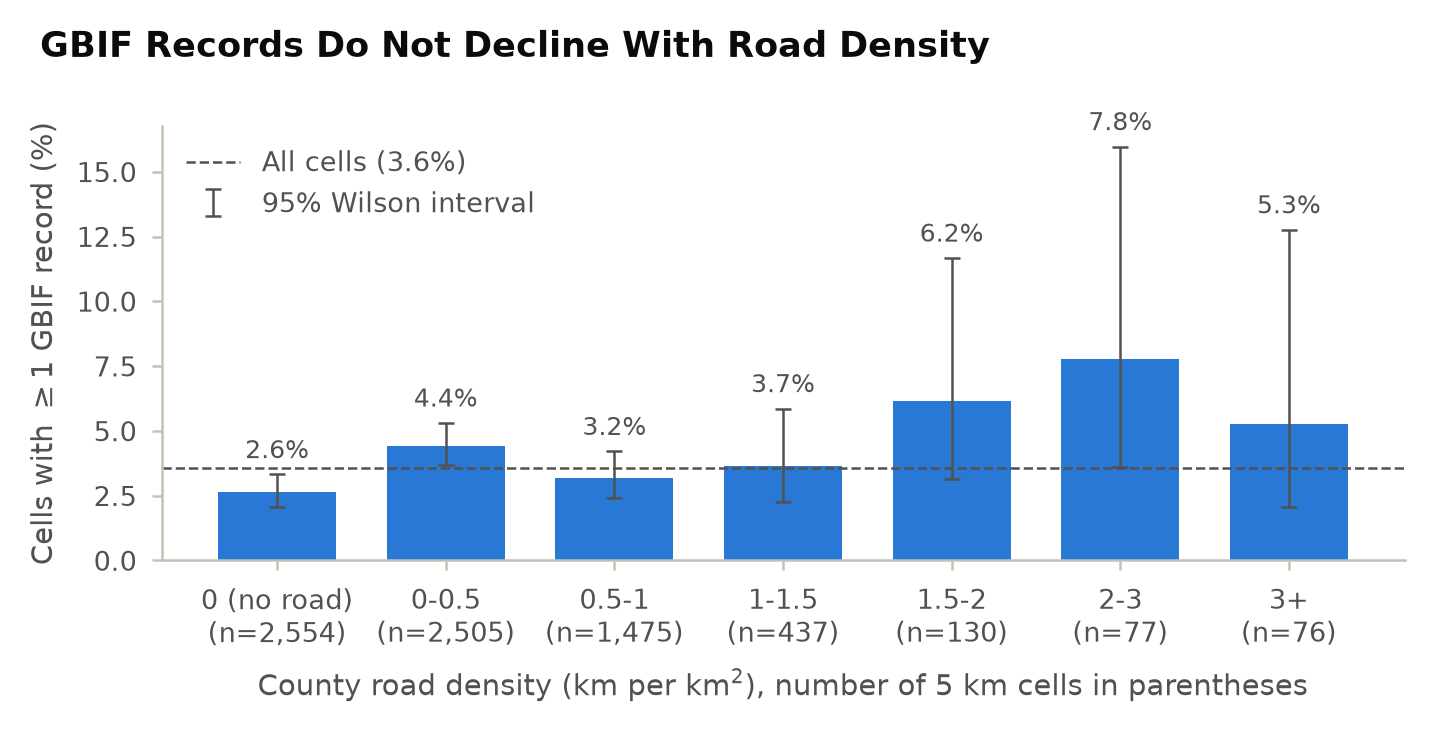
\includegraphics[width=0.75\textwidth]{road_density_vs_presence.png}
  \caption{The share of cells with a GBIF record shows no overall decline as road density rises, so the EDA shows no sign of roads acting as barriers. Error bars are 95\% Wilson intervals; the dashed line is the share across all cells.}
  \label{fig:presence}
\end{figure}

Figure~\ref{fig:presence} previews RQ2. It bins cells by road density and shows the percentage with at least one GBIF record, labeling each bin with its number of cells. I chose this over a scatter plot because 96\% of cells have no record. The share \emph{rises} from 2.6\% in roadless cells to 6--8\% at 1.5--3 km/km$^2$, although the densest bins hold only 76--130 cells and their 95\% intervals (e.g., 3.6--16\% for 2--3 km/km$^2$) overlap the overall 3.6\%. Whatever trend there is runs opposite to the barrier hypothesis and most likely reflects observer bias, so in RQ2 I will read a positive $\rho$ as a sign of reporting effort.

\medskip
\noindent
\textbf{RQ1.} $H_0$: \texttt{dist\_to\_road\_m} has the same distribution for WUI and Wildland records. $H_A$: WUI records are stochastically closer to roads. Tests: Mann--Whitney $U$ (primary) and Welch's $t$-test on $\log(1+d)$ (secondary).

\begin{table}[!htb]
  \centering
  \caption{Assumption checks for RQ1 (\texttt{dist\_to\_road\_m} in meters).}
  \label{tab:assump}
  \begin{tabular}{llrrrrrr}
    \toprule
    Data & Group    & $n$   & Median & SD    & Skew & Shapiro $p$       & Skew of $\log$ \\
    \midrule
    GBIF & WUI      & 116   & 171    & 269   & 2.23 & $1\times10^{-11}$ & $-0.68$        \\
    GBIF & Wildland & 247   & 1,780  & 4,531 & 2.96 & $2\times10^{-21}$ & $-0.79$        \\
    WDFW & WUI      & 4,240 & 35     & 537   & 6.67 & $1\times10^{-77}$ & 0.14           \\
    WDFW & Wildland & 253   & 62     & 3,076 & 5.93 & $2\times10^{-29}$ & 0.18           \\
    \bottomrule
  \end{tabular}
\end{table}

\begin{itemize}
  \item \emph{Normality}: rejected for every group (Table~\ref{tab:assump}). Logs remove most of the skew, so Welch's test is applied only to log-distance, and Mann--Whitney, which needs no normality, is primary. Log-distance is still non-normal (Shapiro $p<10^{-4}$), but with at least 116 records per group Welch's test is robust to this.
  \item \emph{Equal variances}: rejected (Levene $p=1.4\times10^{-10}$ for GBIF, $1.9\times10^{-39}$ for WDFW), so I use Welch rather than Student's $t$-test.
  \item \emph{Similar shape}: the spreads differ (Figure~\ref{fig:box}), so a significant $U$ means WUI records are stochastically closer, not that the medians differ.
  \item \emph{Independence}: doubtful, since one cell holds 24 GBIF records; I will rerun with one record per cell.
\end{itemize}
\noindent
\textbf{RQ2.} $H_0$: Spearman's $\rho=0$ between \texttt{road\_density\_km2} and \texttt{cougar\_count}. $H_A$: $\rho<0$ (barrier). Because the EDA already shows a positive trend, I will also report the two-sided result.
\begin{itemize}
  \item \emph{Paired data}: satisfied, with one density and one count per cell.
  \item \emph{Monotonic relationship}: only partly (Figure~\ref{fig:presence}: weak, noisy, mostly increasing), so I will also report the per-bin shares.
  \item \emph{Ties}: very heavy (96.4\% zero counts, 2,554 zero densities), which makes the asymptotic $p$-value unreliable, so I will use a permutation $p$-value.
  \item \emph{Independence}: violated by spatial autocorrelation; if time allows, I will shuffle within 50 km blocks.
\end{itemize}

\section{Challenge Goals Update}
\begin{description}[leftmargin=0pt, itemsep=2pt]
  \item[New Library.] \texttt{rasterio} reads and samples the WUI raster (WUI class and distance in RQ1, WUI features in RQ3), \texttt{scipy} provides the distance transform and the tests for RQ1 and RQ2, and \texttt{plotly} will draw an interactive RQ2 map. None is taught in CSE 163, and the first two each serve at least two RQs. \texttt{rasterio} and \texttt{scipy} are already in use, and the Plotly map is still to do.
  \item[Result Validity.] Sighting patterns can arise by chance or from observer bias, so each finding gets a test suited to the data. After the EDA, Mann--Whitney became the primary RQ1 test, with Welch on log-distance and the robustness checks in Section~\ref{sec:method}. RQ2 now uses a permutation $p$-value because of heavy ties. Section~\ref{sec:joined} states the hypotheses and checks the assumptions.
  \item[Machine Learning.] RQ3 tunes a Random Forest and an RBF SVM, over hyperparameter grids. Only 3.6\% of cells are positive, so a model that always predicts ``no cougar'' would be 96\% accurate. The plan therefore now uses stratified splits and class weights, and scores models by PR-AUC (the area under the precision-recall curve), which rewards finding the rare positive cells. A model that guesses at random scores a PR-AUC about equal to the positive rate, so the goal is met if the best model's test PR-AUC is clearly above 0.036.
\end{description}

\section{Work Plan Evaluation}
\label{sec:plan}
\begin{table}[!htb]
  \centering
  \caption{Work plan for the rest of the project.}
  \label{tab:plan}
  \begin{tabular}{@{}rlrl@{}}
    \toprule
    \# & Task                                                & Hours & Status               \\
    \midrule
    1  & Download and clean the four datasets                & 1     & Done                 \\
    2  & Per-dataset EDA, spatial joins, and the 5 km grid   & 4     & Done                 \\
    3  & Turn notebooks into modules; write and extend tests & 3.5   & 1.5 h done, 2 h left \\
    4  & RQ1 tests and sensitivity checks                    & 3     & To do                \\
    5  & RQ2 tests, permutation nulls, and Plotly map        & 4     & To do                \\
    6  & RQ3 features, model grids, and evaluation           & 6     & To do                \\
    7  & Final report                                        & 6     & To do                \\
    \midrule
       & Total                                               & 27.5  &                      \\
    \bottomrule
  \end{tabular}
\end{table}

\noindent My proposal budgeted 21.5 h for different data, but the stages line up. Setup took 1 h instead of 0.5 h, because the GBIF API returns only 300 records per request and the road lengths were in degrees. Combining, exploring, and visualizing took 5.5 h of the 10 h budgeted: 3 h of per-dataset EDA (mostly learning to read the 260-million-cell raster), 1 h of spatial joins, and 1.5 h turning notebooks into modules and tests. The proposal had no time for statistical tests or machine learning, so the new plan totals 27.5 h.

\noindent\textbf{Remaining.} About 21 h: 2 h of tests for the new code and 19 h for Tasks 4--7. RQ3 is the least certain estimate, since it may take some time to figure out.

\section{Testing}
\texttt{test\_eda.py} has twelve assert-based tests aimed at errors that give wrong numbers without raising an error: unit mix-ups (feet, meters, and degrees all appear in the data), projections, and clipping. Eleven run the code on small hand-built inputs whose answers I worked out on paper. A point 100 m beside a 1 km road is 100 m from it, and a point past the road's end is measured to the endpoint (a 300--400--500 m triangle). On a 3$\times$3 raster with one WUI cell, the distances are 0, 10, and $10\sqrt{2}$. A 2 km road crossing two 1 km cells gives each a density of exactly 1.0, and a border cell with under 25\% land is dropped. Others cover \texttt{add\_wui\_columns} on a small test GeoTIFF, the WUI code groups, the GBIF filter, the summary functions, the Wilson interval (0.237--0.763 for 5 of 10), and the assumption-check table.

The twelfth test checks the real data: kept GBIF records lie inside Washington and are not fossils, WDFW points lie within 2 km of the outline (which catches a wrong source CRS), \texttt{Incident Type} has exactly three values plus 25 missing, and every raster cell is a class or NoData. Independent totals agree too: the WUI class areas match the state's area, and \texttt{run\_eda.py} and \texttt{test\_eda.py} load the same 396 GBIF records separately. Comparing the 30 m and 120 m rasters exposed a resolution artifact (9 GBIF and 142 WDFW WUI points looked non-WUI), which I fixed, and map overlays (Figure~\ref{fig:incmap}) confirm the layers line up.

\section{Collaboration}
I used the documentation for GBIF's API, \texttt{geopandas}, \texttt{rasterio}, \texttt{scipy}, and \texttt{matplotlib}, plus the WADNR and WSDOT dataset pages. I also read existing Stack Overflow answers about \texttt{rasterio} and about sharing one style across \texttt{matplotlib} figures, which is how I ended up with \texttt{plot\_style.py} to keep the chart code simpler. I am a statistics major so the nonparametric tests (Mann-Whitney, permutation tests), the Wilson interval, and the evaluation metrics for imbalanced classes come from my statistics coursework. Claude was used to help debug figure generation, new package bugs, and to create LaTex tables (such as in appendix, though all the data contained comes from the code).

\appendix
\section{Appendix: WDFW incidents by county and type}
\label{app:counties}
Table~\ref{tab:counties} lists every value of \texttt{County} with its number of incident reports, and Figure~\ref{fig:county} breaks the counts down by \texttt{Incident Type}.

\begin{table}[!htb]
  \centering
  \caption{WDFW cougar incident reports by county, October 2016--July 2022 (4,954 total).}
  \label{tab:counties}
  \begin{tabular}{@{}lr@{\hspace{2.5em}}lr@{\hspace{2.5em}}lr@{}}
    \toprule
    County       & Reports & County    & Reports & County      & Reports \\
    \midrule
    Spokane      & 571     & Benton    & 133     & Walla Walla & 39      \\
    Stevens      & 439     & Pierce    & 129     & Garfield    & 32      \\
    Chelan       & 383     & Skagit    & 128     & Pacific     & 27      \\
    King         & 305     & Kitsap    & 127     & Asotin      & 23      \\
    Grays Harbor & 287     & Clallam   & 127     & Whitman     & 20      \\
    Pend Oreille & 236     & Whatcom   & 112     & Franklin    & 18      \\
    Thurston     & 225     & Jefferson & 108     & Island      & 11      \\
    Okanogan     & 222     & Lincoln   & 84      & Wahkiakum   & 8       \\
    Snohomish    & 212     & Douglas   & 76      & Adams       & 2       \\
    Mason        & 186     & Cowlitz   & 66      & Clark       & 0       \\
    Yakima       & 172     & Ferry     & 63      & Klickitat   & 0       \\
    Kittitas     & 153     & Columbia  & 43      & San Juan    & 0       \\
    Lewis        & 148     & Grant     & 39      & Skamania    & 0       \\
    \bottomrule
  \end{tabular}
\end{table}

\begin{figure}[!htb]
  \centering
  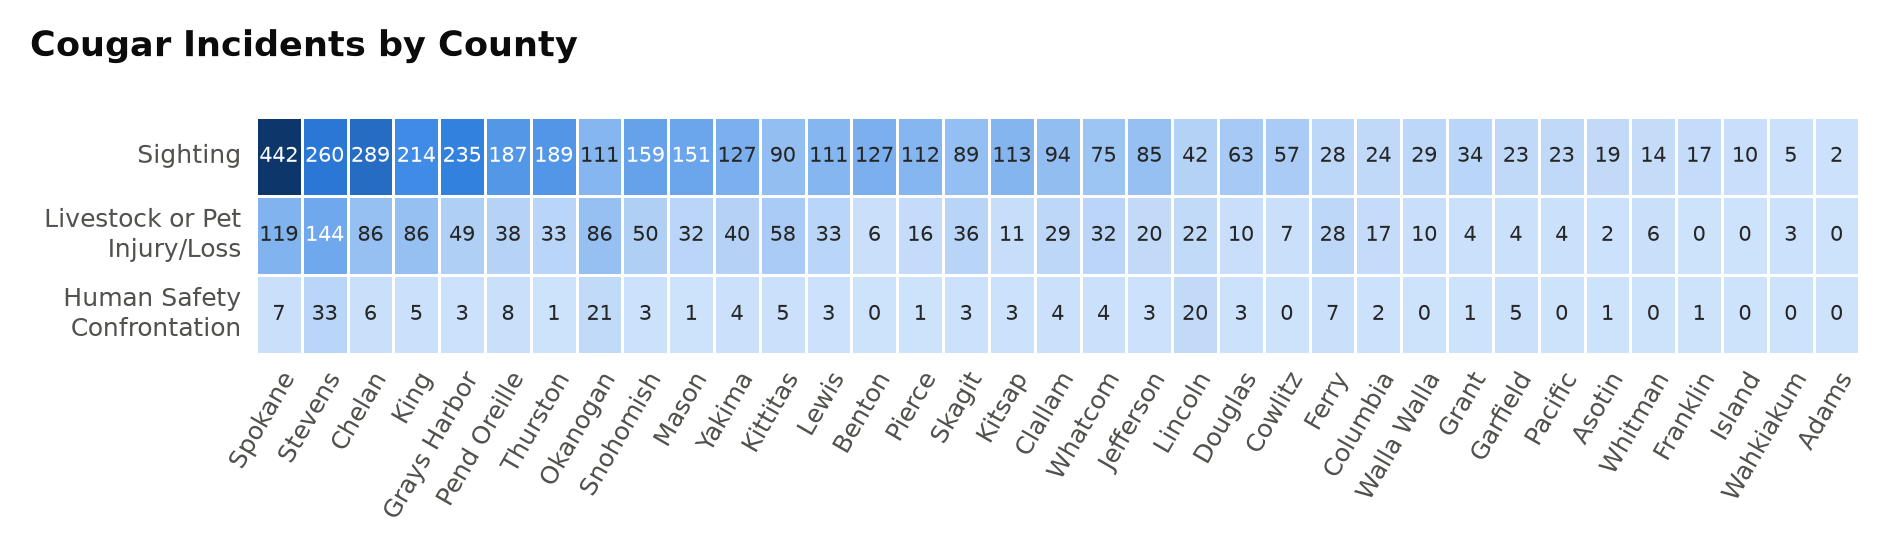
\includegraphics[width=\textwidth]{incidents_by_county.png}
  \caption{Spokane, Stevens, and Chelan report the most incidents, and conflict types concentrate in a few counties.}
  \label{fig:county}
\end{figure}
Figure~\ref{fig:county} is a heatmap of counts by \texttt{County} (sorted by total) and \texttt{Incident Type}, which shows both categorical variables at once with exact counts. Stevens County leads in livestock/pet losses (144) and human-safety confrontations (33), and Okanogan and Lincoln have unusually many confrontations for their number of reports.
\end{document}
